% Kapitel 3 mit den entsprechenden Unterkapiteln
% Die Unterkapitel können auch in separaten Dateien stehen,
% die dann mit dem \include-Befehl eingebunden werden.
%------------------------------------------------------------------------------------
\chapter{Resultierende Softwarearchitektur}

Dieser Abschnitt hat die Aufgabe, einen Überblick über die zu entwickelnden
Komponenten und Subsysteme zu liefern.
\section{Komponentenspezifikation}

In diesem Abschnitt wird die aus der Analyse der Produktfunktionen (Kapitel 2)
resultierende Komponentenstruktur zunächst überblickartig durch ein
Komponentendiagramm beschrieben. Die Bezeichnungen und Anzahl der Komponenten
muss natürlich konsistent sein mit der in Kapitel 2!

\begin{figure}[h]
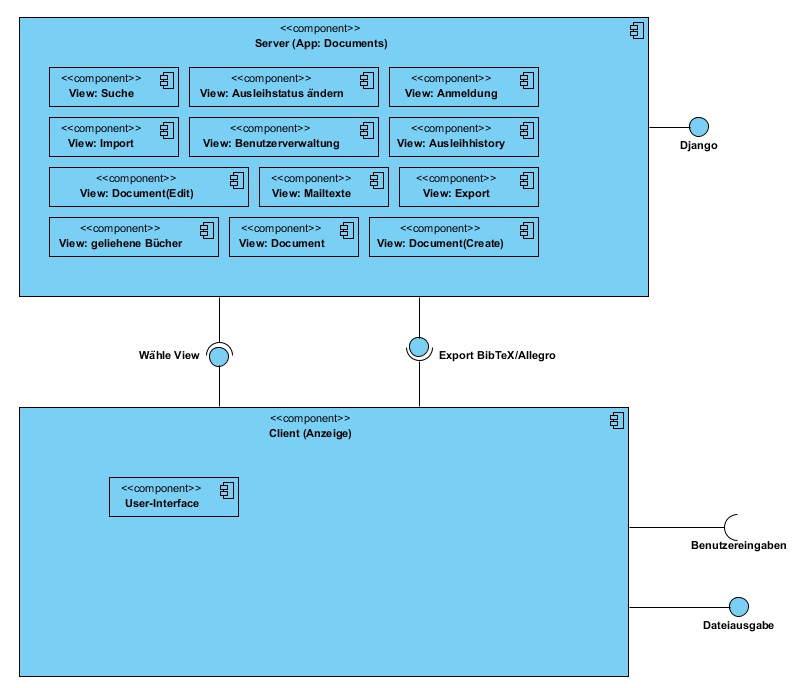
\includegraphics[width=0.8\linewidth]{bilder/komponentendiagramm_client_server.jpg}
\caption[Komponentendiagramm]{Komponentendiagramm}
\label{Komponentendiagramm}
\end{figure}

\section{Schnittstellenspezifikation}

\begin{tabular}[ht]{|l|p{0.35\linewidth}|p{0.35\linewidth}|}
\hline
Schnittstelle & \multicolumn{2}{|c|}{Aufgabenbeschreibung}\\
\hline
\hline
/S10/ Wähle View & \multicolumn{2}{|c|}{}\\
\hline
& search(String) : List & Die Suche liefert eine Liste mit den Ergebnissen\\
& signIn(String) : boolean & Anmelden des Benutzers\\
& signOut() : boolean & Abmelden des Benutzers\\
& import(data) : boolean & Import \\
& getRole(String) : String & liefert die aktuelle Rolle des Nutzers\\
& getHistory(String) : List & liefert eine Liste der Ausgeliehen Dokumente\\
& getDoc(String) : List & liefert die Dokumentinformationen in einer Liste\\
& getLend(String) : String & liefert den Nutzernamen der das Dokument ausgeliehen hat\\
\hline
/S20/Export & \multicolumn{2}{|c|}{Exportieren von Informationen}\\
\hline
& exportBibTeX() : String & Liefert einen String welcher die Dokumentinformationen im BibTeX-Format enthält\\
& exportAllegro() : & Liefert eine Datei für die UB\\
\hline
/S30/Django & \multicolumn{2}{|c|}{Verbindung mit Datenbank}\\
\hline
& connect(String) : boolean & Verbindung zur Datenbank\\
& disconnect() : boolean & Verbindung wird beendet\\
& sendQuery(String) : List & liefert eine Liste des Ergebnisses\\
\end{tabular}





\section{Protokolle für die Benutzung der Komponenten}

In diesem Abschnitt wird mit Hilfe von Protokoll-Statecharts die korrekte
Verwendung der zu entwickelnden Komponenten dokumentiert. Dies ist insbesondere
für diejenigen Komponenten notwendig, für die eine Wiederverwendung möglich
erscheint oder sogar bereits geplant ist.

Begründen Sie für welche Komponenten eine Wiederverwendung sinnvoll erscheint
und für welche nicht!

Fügen Sie so viele Statechartdiagramme ein, wie sie Komponenten gefunden haben.
